In the model we investigate here, there are $L$ unlinked causal loci at which
mutations influence the trait value. An infinite number of mutation are possible
within each locus and the mutation rate per unit of coalescent time to mutations
affecting the trait is $\T$. That is, $\T$ is the mutation rate for the entire
locus and not necessarily per nucleotide. Mutations are randomly assigned
effects from a distribution of effect sizes, and effects are additive both
within and between loci. The moment generating function (mgf) of this
distribution is written as $\psi$ and the $i^{th}$ (non-central) moment is
$m_i$. The sum of all mutations occurring in a haploid individual's history
determines the trait value of the individual. Correlations between individuals
arise when mutations fall on shared portions of genealogies at specific loci.
Because the loci are unlinked we assume their genealogies are independent. This
model is shown schematically in Figure \ref{fig:schema}.

The genealogy at a locus is represented by the random vector of branch lengths,
$\mathbf{T}$. An element $T_{\omega}$ of $\mathbf{T}$ is the branch length
subtending only individuals in the set $\omega$ and no others in the sample. For
example, $T_{\{a,b\}}$ is the length of the branch subtending only individuals
$a$ and $b$. If a branch subtending only $a$ and $b$ does not exist for a given
genealogy $T_{\{a,b\}}$ is set to zero. In this way $\mathbf{T}$ encodes both
the branch lengths and the topology of a genealogy. $\Omega$ is the set of all
possible branches. If there are three sampled individuals, $a$, $b$, and $c$,
then $\Omega=\{\{a\},\{b\},\{c\},\{a,b\},\{a,c\},\{b,c\}\}$ and
$\mathbf{T}=(T_{\{a\}},T_{\{b\}},T_{\{c\}},T_{\{a,b\}},T_{\{a,c\}},T_{\{b,c\}})$.
The mgf for the distribution of trait values is denoted $\varphi_{\mathbf{T}}$.

Phenotypic trait values are the random quantities we are interested in and
result from mutations occuring along the branches of genealogies. We will
hereafter refer to the phenotypic trait simply as trait values and ignore any
environmental component. Starting with a trait controlled by a single locus, the
random vector of trait values in the sampled individuals is $\mathbf{Y}$, such
that for sampled individuals $a$, $b$, and $c$, $\mathbf{Y}=\{Y_a,Y_b,Y_c\}$.
The trait values are modeled as the change relative to the value in the most
recent common ancestor (MRCA) of the sample at that locus. Since we do not know
the ancestral value, we cannot be directly observe the change in trait values.
Thus, for a trait controlled by multiple loci, $\mathbf{Y}$ is the sum over
contributions from these loci, each measured with respect to an arbitrary value.
However, $\mathbf{Y}$ is sufficient to determine measurable quantities such as
differences in trait values between individuals and the sample variance. The
moment generating functions for the distribution of branch lengths is denoted as
$\varphi_{\mathbf{Y}}$.

\begin{figure}
  \centering
  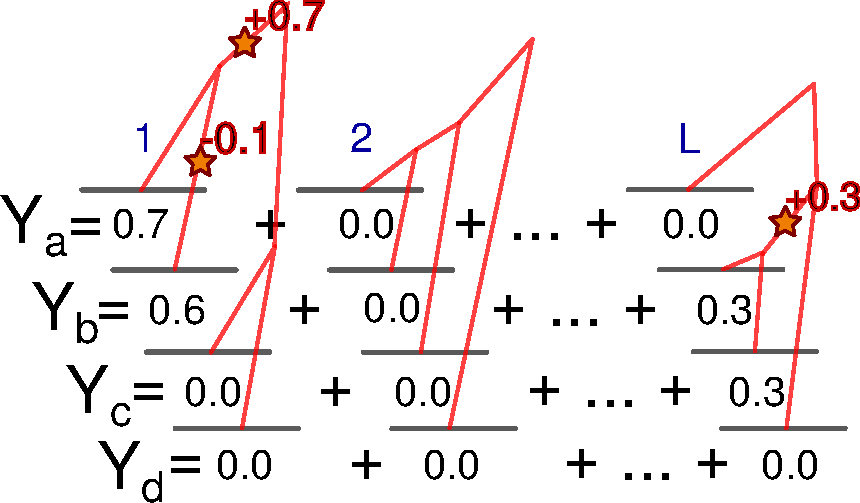
\includegraphics[width=0.8\textwidth]{figures/schema.pdf}
  \caption{A schematic representation of the model analyzed.
  $L$ loci affect the trait in a set of individuals and have independent
  genealogies. Mutations occur within loci as a Poisson process and act
  additively to give individual trait values. Potentially many loci affecting
  the trait may receive no mutations.}
  \label{fig:schema}
\end{figure}

Here we refer to the genetic architecture of a trait as the combination of
genetic parameters affecting the trait distribution ($L$, $\T$, $\psi$).
Therefor, the realized distribution for a given genetic architecture is a random
quantity. Another useful way to describe a trait is by its sparsity, how many
segregating mutations influence the trait. A more `sparse' trait is affected by
fewer mutations. Formally, we measure sparsity as the average number of pairwise
differences separating two randomly chosen haplotypes at loci affecting the
trait. Sparsity thus depends both on the genetic architecture through the
mutation rate, the number of causal loci, and the distribution of coalescence
times.

For populations of exchangeable individuals a concise way to summarize the
distribution of genealogies is $\mathbbm{T}_{i,j}$ which gives the amount of
time that $i$ lineages remain in the genealogy of a a sample of size $j$. The
pairwise coalescent time between a lineage in individual $i$ and in individual
$j$ is written as $\mathcal{T}_{i,j}$. When considering structured populations
$\mathcal{T}_{a,b}$ is also used to denote the coalescence time between a
randomly chosen lineage from subpopulation $a$ and a randomly chosen lineage
from subpopulation $b$. A final set of quantities are defined for sums of branch
lengths. Let $\tau_{a+b}$ be the sum of all branches ancestral to both $a$ and
$b$, and $\tau_{a/b}$ be the sum of all branches ancestral to $a$ but not $b$.
Extensions of this for more than two individuals are also used. The same
notation is used when referring to sets of branch indices. So $\Omega_{a+b}$ and
$\Omega_{a/b}$ would be the sets of branches summed to give $\tau_{a+b}$ and
$\tau_{a/b}$ respectively.

%%% Local Variables:
%%% TeX-master: "short_report.tex"
%%% End:
